\documentclass[12pt,a4paper]{report}

\usepackage{csquotes}
\usepackage[croatian]{babel}
\usepackage{amsmath, amsthm, amssymb}
\usepackage{epsfig}
\usepackage{graphicx}
\usepackage{hyperref}
\usepackage[left=3.5cm,top=1.5cm,right=3cm,bottom=4cm]{geometry}
\usepackage{mathtools}
\usepackage{bookmark}

\usepackage[backend=biber,style=numeric]{biblatex}
\addbibresource{ref.bib}

\usepackage{fancyhdr}
\pagestyle{fancy}

\usepackage[T1]{fontenc}
% Fonts:
\usepackage{helvet} % Helvetica; phv
\usepackage{palatino} % Palatino; ppl

\gdef \title{Seminarski rad}
\gdef \class{Matematika 3}
\gdef \author{Tin Švagelj}
\gdef \degree{Jednopredmetna Informatika}
\gdef \university{
Fakultet Informatike i Digitalnih Tehnologija\\
Rijeka
}
\gdef \semguide{dr.sc. Marija Maksimović}
\gdef \author{Tin Švagelj}
\gdef \date{\today}

\graphicspath{{./figures/}}

\newcommand{\UseFont}[1]{\fontfamily{#1}\selectfont}

% \usepackage{fancyhdr}
% \pagestyle{fancy}
% \fancyhead{}
% \renewcommand\headrulewidth{0.1pt}
% \fancyhead[L]{\footnotesize \leftmark}
% \fancyhead[R]{\footnotesize \thepage}
% \renewcommand\headrulewidth{0pt}
% \fancyfoot[R]{\small Fakultet Informatike i\\Digitalnih Tehnologija}
% \renewcommand\footrulewidth{0.1pt}
% \fancyfoot[C]{2022 - 2023}
% \fancyfoot[L]{\small \title}

\begin{document}

\thispagestyle{empty}
\begin{titlepage}
	\begin{center}
		\vspace*{20pt}
		{\UseFont{phv} \Large \bf \title \par}
		{\large \em \UseFont{pzc} za kolegij \UseFont{phv} \class}\\ [.15\baselineskip] \par

		\vspace{\stretch{0.3}}

		voditeljica kolegija:\\
		{\bf \semguide},\\
		\vspace*{10pt}
		student:\\
		{\bf \author}\\
		\UseFont{ppl} {\bfseries \degree}

		\vspace{\stretch{0.25}}
		
		\footnotesize{\bf \university} \par
		\bf{\date}
	\end{center}
\end{titlepage}

\pagenumbering{roman}

\tableofcontents

\newpage

\setcounter{page}{1}
\pagenumbering{arabic}

\chapter{Uvod}

Potrebno je odrediti ekstreme i nacrtati funkciju:
\begin{equation}
f(x, y) = 2x^3 + 2y^3 - 36xy + 430
\end{equation}

Kako bismo mogli odrediti ekstreme multivarijatne funkcije, potrebno je odrediti domenu funkcije.

Zatim je potrebno odrediti parcijalnu derivaciju prvog reda multivarijatne funkcije,
pri čemu (u ovom slučaju) koristimo pravila deriviranja \cite{mzi}:

\begin{align}
    (c)' &= 0 \text{ i }\\
    (x^a)' &= ax^{a-1}.
\end{align}

, i pravilo o deriviranju zbroja \cite{mzi}:

\begin{equation}
    (f + g)' = f' + g'.
\end{equation}

Sa parcijalnom drivacijom prvog reda funkcije $f$ po $x$ i drivacijom prvog reda po $y$ određujemo stacionarne točke, rješavajući sustav jednadžbi:
\begin{equation}
    \begin{cases}
        \frac{\partial f}{\partial x} = 0 \\
        \frac{\partial f}{\partial y} = 0
    \end{cases}
\end{equation}

Kako bi utvrdili jesu li dobivene točke sedlaste, minimumi ili maksimumi, potrebna nam je derivacija drugog reda:

\begin{equation}
    \frac{\partial^2 f}{\partial x^2} = \frac{\partial}{\partial x} (\frac{\partial f}{\partial x}).
\end{equation}

Za računanje Hessove matrice također nam je potrebna derivacija $f$ po $x$ i $y$:

\begin{equation}
    \frac{\partial^2 f}{\partial x \partial y} = \frac{\partial}{\partial y} (\frac{\partial f}{\partial x}).
\end{equation}

Za neku funkciju $f(x, y)$, Hessova matrica je definirana kao
$\mathbf{H}(f(\mathbf{x, y})) = \mathbf{J}(\nabla f(\mathbf{x, y}))$,
gdje je gradijent ($\nabla$) funkcije $f$:

\begin{equation}
    \nabla f(\mathbf{x}, \mathbf{y}) = \begin{bmatrix}
        \frac{\partial f}{\partial x} \\
        \frac{\partial f}{\partial y}
    \end{bmatrix}
\end{equation}

Dakle Hessova matrica funkcije $f(x, y)$ je:
\begin{equation}
    \mathbf H_f= \begin{bmatrix}
        \dfrac{\partial^2 f}{\partial x_1^2} & \dfrac{\partial^2 f}{\partial x_1\,\partial x_2}\\
        \dfrac{\partial^2 f}{\partial x_2\,\partial x_1} & \dfrac{\partial^2 f}{\partial x_2^2}
    \end{bmatrix}.
\end{equation}

\chapter{Razrada}

S obzirom da je zadana multivarijatna funkcija polinom, važeća za svaki $x \in \mathbb{R}$ i $y \in \mathbb{R}$.
Dakle domena funkcije je skup svih realnih brojeva:
$$
    D(f) = \mathbb{R} \times \mathbb{R} = \mathbb{R}^2
$$

\section{Parcijalne derivacije prvog reda}

\begin{align*}
    \frac{\partial f}{\partial x} & = \frac{\partial}{\partial x} (2x^3 + 2y^3 - 36xy + 430) \\
    & = \frac{\partial}{\partial x} 2x^3 + \frac{\partial}{\partial x}2y^3 - \frac{\partial}{\partial x}36xy + \frac{\partial}{\partial x}430 \\
    & = 6x^2 + 0 - 36y + 0 \\
    & = 6x^2 - 36y \\
    \\
    \frac{\partial f}{\partial y} & = \frac{\partial}{\partial y} (2x^3 + 2y^3 - 36xy + 430) \\
    & = \frac{\partial}{\partial y} 2x^3 + \frac{\partial}{\partial y}2y^3 - \frac{\partial}{\partial y}36xy + \frac{\partial}{\partial y}430 \\
    & = 0 + 6y^2 - 36x + 0\\
    & = 6y^2 - 36x
\end{align*}

\section{Stacionarne točke}

$$
\begin{cases}
    6x^2 - 36y = 0 \\
    6y^2 - 36x = 0
\end{cases}
$$

Izrazimo $y$ iz prvog izraza,
\begin{align*}
    6x^2 - 36y &= 0 \\
    36y & = 6x^2 \\
    y & = \frac{6x^2}{36} = \frac{x^2}{6} \\
\end{align*}

te ga uvrstimo u drugi:
\begin{align*}
    6(\frac{x^2}{6})^2 - 36x & = 0 \\
    x^4 - 36x & = 0
\end{align*}

, jedno rješenje $x_1 = 0$ dobivamo izlučivanjem $x$a iz izraza:
\begin{align*}
    x(x^3 - 36) &= 0 \\
    x_1 &= 0
\end{align*}

drugi član umnoška nam daje drugo rješenje:
\begin{align*}
    x^3 - 36 &= 0 \\
    x^3 &= 36 \\
    x &= \sqrt[3]{36} \\
    x_2 &= \sqrt[3]{36},
\end{align*}

zbog duplog pojavljivanja $x$a u zadanom polinomu se radi o funkciji simetričnoj s obzirom na ishodište te trebamo tretirati drugo rješenje kao da je njegov predznak uklonjen.

Tom logikom dobivamo 3 rješenja sustava:
\begin{center}
\begin{tabular}{c c c}
    $x_1 = 0$ & $x_2 = \sqrt[3]{36}$ & $x_3 = -\sqrt[3]{36}$\\
\end{tabular}
\end{center}

\begin{align*}
    6x^2 - 36y &= 0\\
    6(\sqrt[3]{36})^2 - 36y &= 0\\
    36y &= 6(\sqrt[3]{36^2})\\
    6y &= \sqrt[3]{36^2} \\
    y &= \frac{\sqrt[3]{6^4}}{6} \\
    y &= 6^{\frac{4}{3}} * 6^{-1} = 6^{\frac{4}{3}} * 6^{-\frac{3}{3}} = 6^{\frac{4}{3} - \frac{3}{3}} \\
    y &= \sqrt[3]6 \\
\end{align*}

\begin{center}
\begin{tabular}{c c}
    $x$ & $y$ \\
    $0$ & $0$ \\
    $\sqrt[3]{36}$ & $\sqrt[3]6$ \\
    $-\sqrt[3]{36}$ & $-\sqrt[3]6$ \\
\end{tabular}
\end{center}

\section{Parcijalne derivacije drugog reda}

\begin{align*}
    \frac{\partial^2 f}{\partial x^2} & = \frac{\partial}{\partial x} (6x^2 - 36y)\\
    & = \frac{\partial}{\partial x} 6x^2 - \frac{\partial}{\partial x} 36y\\
    & = 12x - 0\\
    & = 12x\\
    \\
    \frac{\partial^2 f}{\partial y^2} & = \frac{\partial}{\partial x} (6y^2 - 36x)\\
    & = \frac{\partial}{\partial y} 6y^2 - \frac{\partial}{\partial y} 36x\\
    & = 12y - 0\\
    & = 12y\\
    \\
    \frac{\partial^2 f}{\partial x \partial y} & = \frac{\partial}{\partial y} (6x^2 - 36y) \\
    & = \frac{\partial}{\partial y} 6x^2 - \frac{\partial}{\partial y} 36y \\
    & = 0 - 36 \\
    & = -36
\end{align*}

Određujemo vrijednost druge parcijalne derivacije svake stacionarne točke kako bi mogli odrediti Hessovu matricu:

$$H_f = \begin{bmatrix} 12x & -36 \ -36 & 12y \end{bmatrix}$$

Određujemo svojstvene vrijednosti Hessove matrice za svaku stacionarnu točku:

%\begin{itemize}
%    \item Za (0, 0), svojstvene vrijednosti su 0 i 12; dobivena stacionarna točka sedlasta.
%    \item Za (3, 3), svojstvene vrijednosti su 12 i 12; stacionarna točka je lokalni maksimum.
%    \item Za (-3, -3), svojstvene vrijednosti su 12 i 12; stacionarna točka je lokalni minimum.
%\end{itemize}

%Dakle, na osnovu prethodnog računa zaključujemo da su ekstremi funkcije $2x^3 + 2y^3 - 36xy + 430$ točke
%\begin{itemize}
%    \item (3, 3) kao lokalni maksimum
%    \item i (-3, -3) kao lokalni minimum.
%\end{itemize}

Korištenjem \verb|numpy| i \verb|matplotlib| biblioteka u Pythonu, pomoću sljedećeg koda možemo dobiti 3D prikaz cijele multivarijatne funkcije:

\begin{verbatim}
    import numpy as np
    import matplotlib.pyplot as plt
    from mpl_toolkits.mplot3d import Axes3D
    
    def f(x, y):
        return 2*x**3 + 2*y**3 - 36*x*y + 430
    
    x = np.linspace(-10, 10, 100)
    y = np.linspace(-10, 10, 100)
    X, Y = np.meshgrid(x, y)
    Z = f(X, Y)
    
    fig = plt.figure()
    ax = fig.add_subplot(111, projection='3d')
    ax.plot_surface(X, Y, Z)
    
    plt.show()
\end{verbatim}

\noindent\makebox[\textwidth]{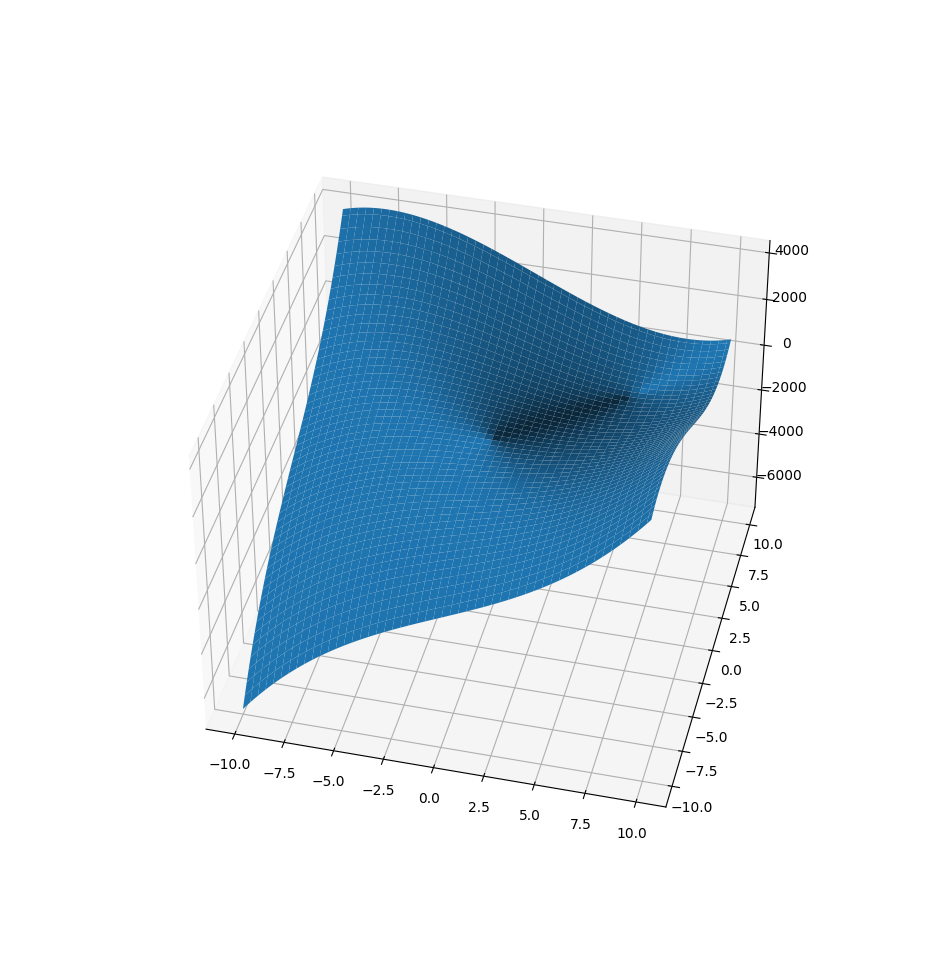
\includegraphics[width=300px]{f_graph}}
\newpage

\chapter{Zaključak}

\newpage

\pagenumbering{roman}
\setcounter{page}{2}

\printbibliography[heading=bibintoc,title=Literatura]

\end{document}
